\documentclass[conference,a4paper]{IEEEtran}
\IEEEoverridecommandlockouts
\usepackage[utf8]{inputenc}
\usepackage[T1]{fontenc}
\usepackage[spanish,es-tabla]{babel}
\usepackage{graphicx,booktabs,amsmath,amssymb}
\usepackage[caption=false,font=footnotesize]{subfig}
\usepackage{listings,xcolor}
\usepackage{cite}
\usepackage[hidelinks]{hyperref}
\lstset{basicstyle=\ttfamily\scriptsize,breaklines=true,frame=single,backgroundcolor=\color{gray!8},columns=fullflexible}

\begin{document}

\title{Kakuro: de la imagen a la solución mediante visión computacional y programación con restricciones}

\author{
\IEEEauthorblockN{Bruno Medina Agnini, Eduardo Bravo, Ricardo Victor Ambrocio Tantalean}
\IEEEauthorblockA{\textit{CC58 -- Tópicos en Ciencias de la Computación}\\
\textit{Universidad Peruana de Ciencias Aplicadas (UPC)}\\
Lima, Perú}
}

\maketitle

\begin{abstract}
Presentamos un sistema que recibe la fotografía o imagen digital de un Kakuro, extrae su estado inicial con visión computacional
y una red neuronal convolucional (CNN) propia, lo resuelve con un modelo de programación con restricciones (CP) en CP-SAT de OR-Tools
y dibuja la solución sobre la imagen original. La extracción combina corrección de perspectiva, segmentación de la grilla por perfiles
de líneas, clasificación de celdas con umbrales locales y una CNN entrenada sólo con datos sintéticos; las reglas del Kakuro y el propio
modelo CP validan la lectura y corrigen errores del OCR. El modelo CP tiene una variable por celda blanca, con el dominio podado por las
combinaciones posibles de sus dos corridas, y en cada corrida las restricciones globales \texttt{AllDifferent} y de suma; una variante con
restricciones de tabla sirve de comparación. Sobre 55 imágenes de prueba, el sistema extrae todas las pistas de 33 imágenes digitales,
simuladas y capturas de una aplicación, y el 95.6\% de las pistas de 22 fotos de celular de tableros impresos tomadas en seis condiciones
(frontal, ángulo, poca luz, sombra, hoja volteada y flash), con 18 de 22 tableros exactos y resueltos. Los 23 tableros con solución única
que usamos se resuelven, con prueba de unicidad, en milisegundos y sólo con propagación, sin ramificar.
\end{abstract}

\begin{IEEEkeywords}
Kakuro, visión computacional, OCR, redes neuronales convolucionales, programación con restricciones, restricciones globales, CP-SAT
\end{IEEEkeywords}

\section{Introducción}
El Kakuro es un pasatiempo numérico que se modela de forma natural como un problema de satisfacción de restricciones (CSP)~\cite{rossi}:
cada celda blanca es una variable con valores del 1 al 9, y cada corrida exige que sus dígitos sumen la pista y sean distintos.
El trabajo pide un sistema \emph{end-to-end} en tres fases: (1)~extraer el estado inicial desde una imagen con visión computacional e IA;
(2)~resolverlo con un modelo CP en OR-Tools; y (3)~integrar ambas partes y mostrar la solución sobre la imagen. Nuestras contribuciones son:
\begin{itemize}
  \item Un pipeline de visión robusto a fotos reales (perspectiva fuerte, hoja girada o volteada, papel curvado, sombras y distintos
        estilos visuales), con una CNN entrenada sólo con datos sintéticos (\emph{domain randomization}).
  \item Un modelo CP con dominios podados y restricciones globales (\texttt{AllDifferent} y suma lineal), comparado con una variante de
        restricciones de tabla.
  \item Una integración en la que la Fase~2 valida a la Fase~1: las sumas imposibles, la orientación de la hoja y las lecturas sin
        solución se resuelven con las reglas del Kakuro y con el propio solver.
  \item Un conjunto de prueba de 55 imágenes en cinco grupos, que incluye 22 fotos reales de tableros impresos con una referencia
        independiente del pipeline.
\end{itemize}

\section{Problema}
Un Kakuro es una grilla con celdas blancas, a rellenar con dígitos del 1 al 9, y celdas negras. Algunas celdas negras están divididas
por una diagonal y contienen pistas: el número del triángulo inferior izquierdo es la suma de la corrida vertical que empieza debajo,
y el del triángulo superior derecho, la de la corrida horizontal a la derecha. Una \emph{corrida} es una secuencia maximal de celdas
blancas contiguas en una fila o columna: sus dígitos suman la pista y no se repiten. Como sólo hay nueve dígitos, una corrida tiene a lo
más 9 celdas, y una de $n$ celdas sólo admite sumas entre $1+\dots+n=n(n+1)/2$ y $9+\dots+(10-n)=n(19-n)/2$. Cada celda blanca
pertenece a exactamente una corrida horizontal y una vertical, por lo que la primera fila y la primera columna nunca tienen celdas
blancas. Un Kakuro bien planteado tiene una única solución.

\section{Fase 1: visión computacional e IA}
La Fig.~\ref{fig:pipeline} muestra las etapas del pipeline sobre una de las imágenes de prueba.

\begin{figure*}[!t]
\centering
\subfloat[Binarización adaptativa]{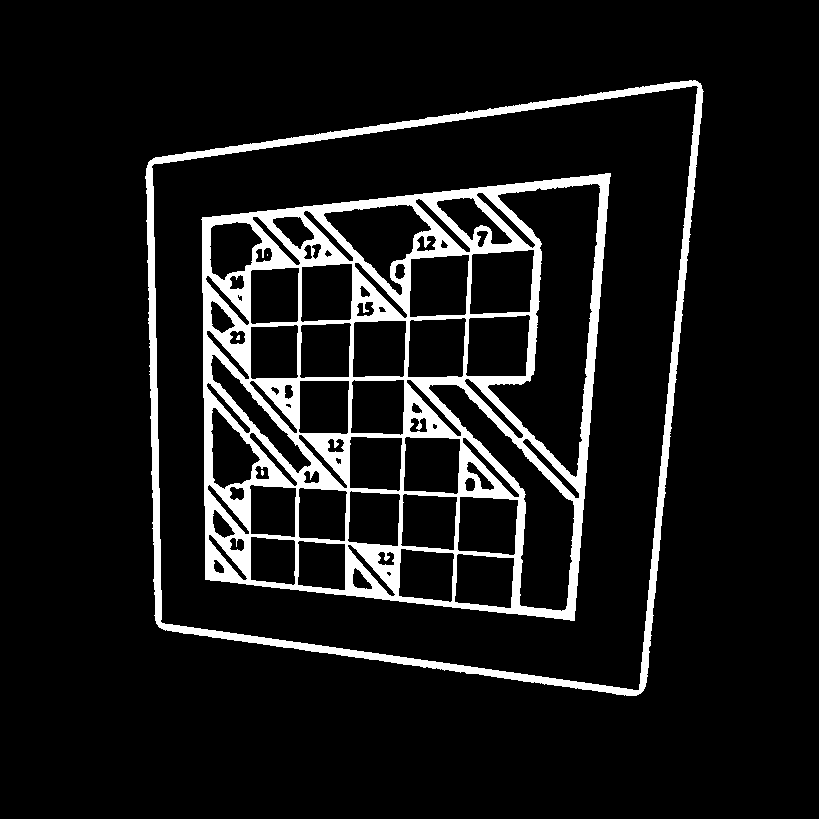
\includegraphics[width=0.31\textwidth]{figs/binary.png}}\hfil
\subfloat[Tablero y esquinas]{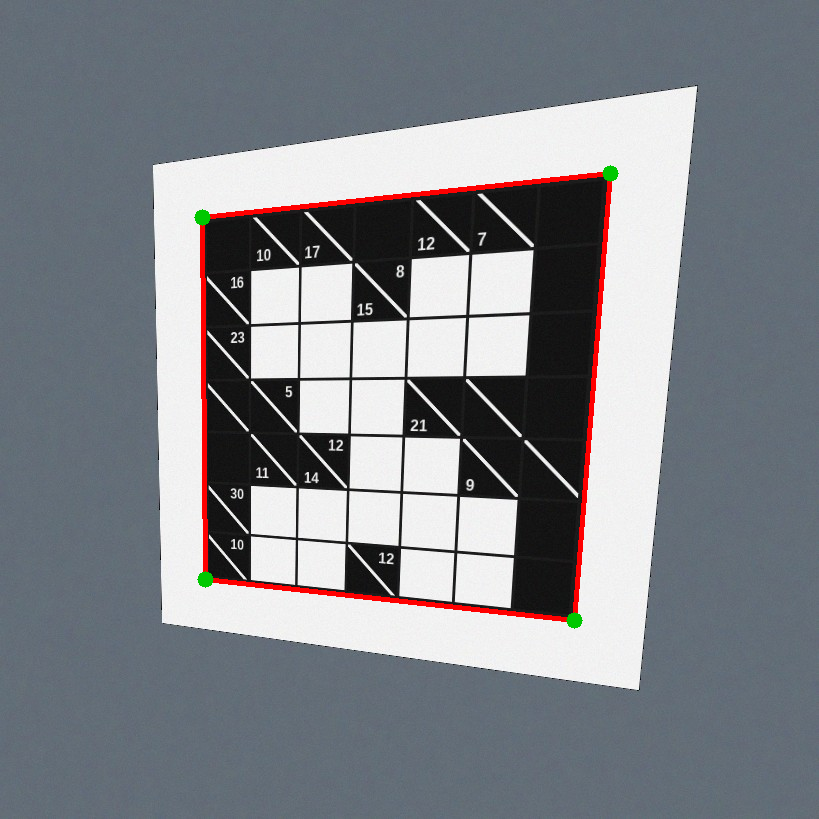
\includegraphics[width=0.31\textwidth]{figs/board.png}}\hfil
\subfloat[Rectificado + grilla]{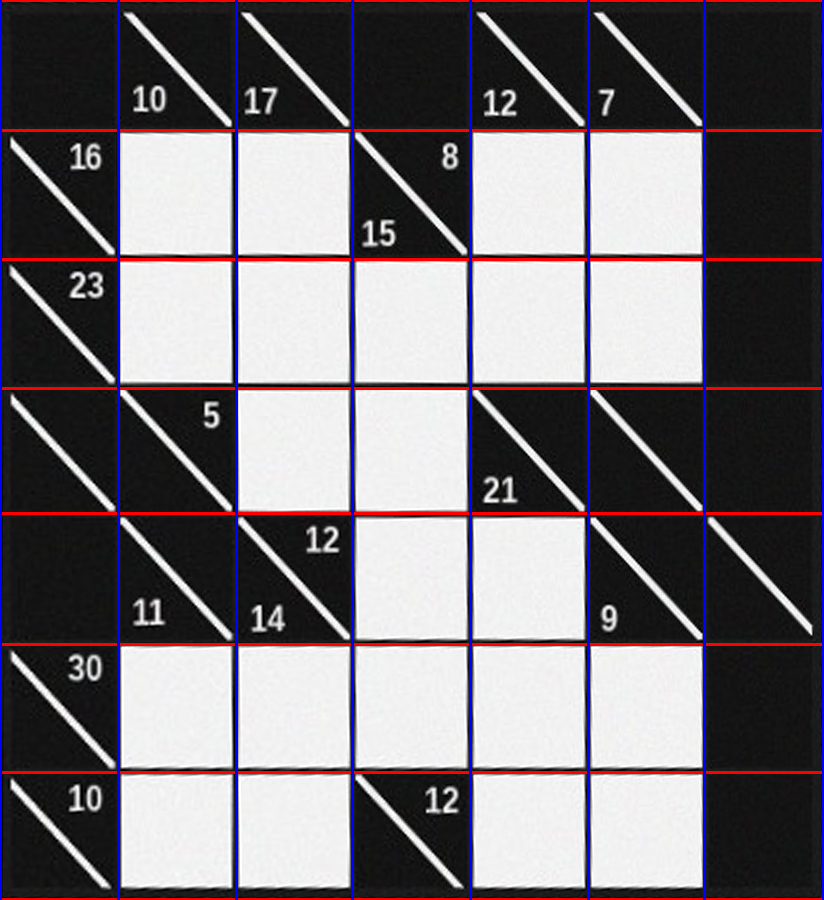
\includegraphics[width=0.31\textwidth]{figs/grid.png}}\\
\subfloat[Clasificación de celdas]{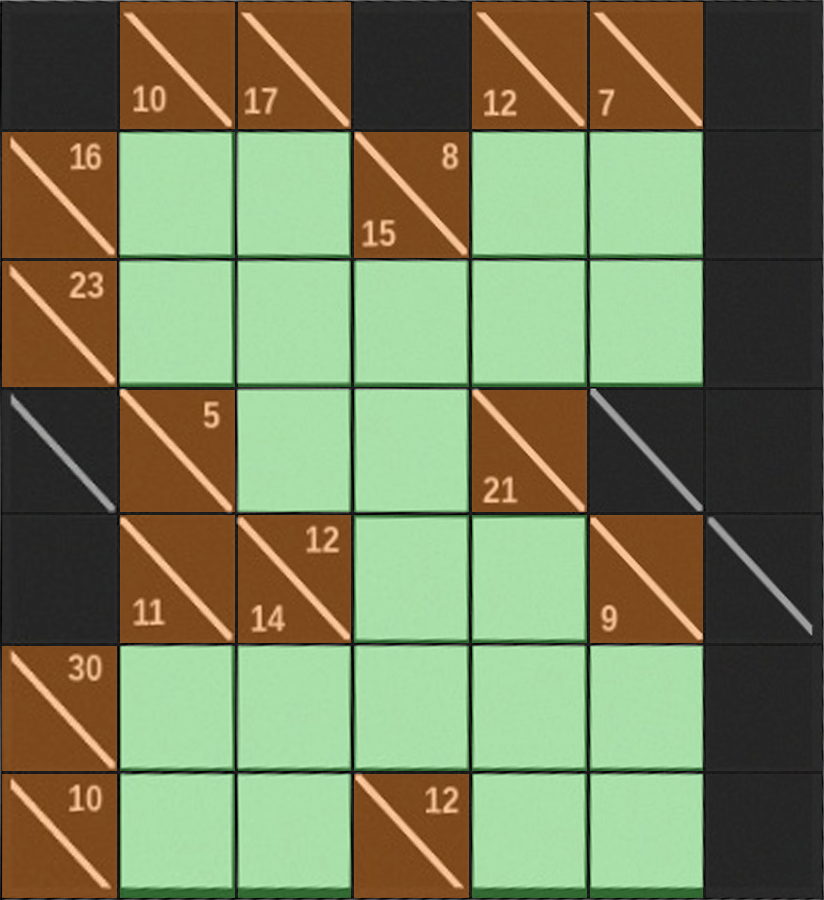
\includegraphics[width=0.31\textwidth]{figs/cells.png}}\hfil
\subfloat[Dígitos 28$\times$28]{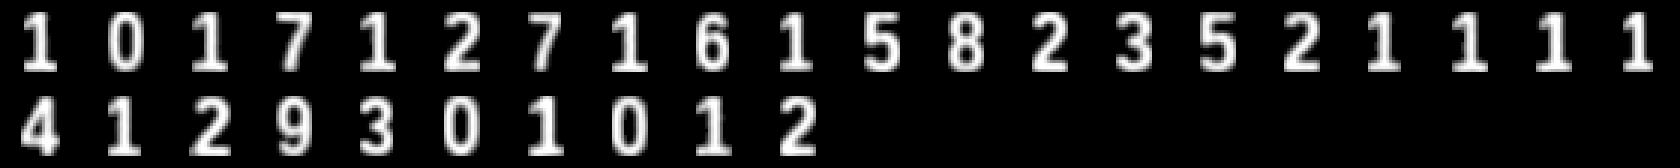
\includegraphics[width=0.31\textwidth]{figs/digits.png}}\hfil
\subfloat[Solución sobre la foto]{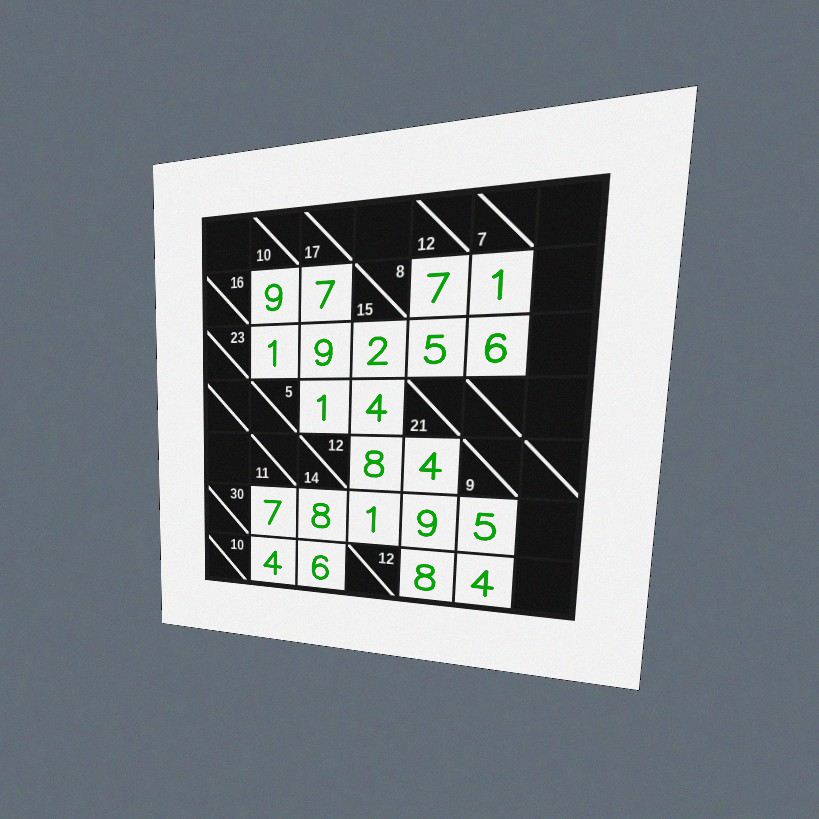
\includegraphics[width=0.31\textwidth]{figs/solution.png}}
\caption{Etapas del pipeline sobre una imagen simulada con ángulo fuerte (\texttt{s05\_angulo\_fuerte}).}
\label{fig:pipeline}
\end{figure*}

\subsection{Preprocesamiento y corrección de perspectiva (\texttt{vision/preprocess.py})}
\begin{enumerate}
  \item Conversión a escala de grises y desenfoque gaussiano $5\times5$ (OpenCV~\cite{opencv}).
  \item Binarización adaptativa gaussiana invertida (bloque $\approx$ lado/30): robusta a iluminación no uniforme, a diferencia de un umbral global.
  \item Localización del tablero como la \emph{componente conexa con más píxeles de tinta} (líneas y bordes de celdas negras).
        Elegir la componente y no el contorno más grande evita confundir el tablero con el borde de la hoja cuando la foto se toma sobre una mesa.
        Si el tablero toca el borde de la imagen (captura recortada) se usa la imagen completa.
  \item Esquinas: envolvente convexa de la componente y \texttt{approxPolyDP} hasta obtener 4 vértices (respaldo: \texttt{minAreaRect}),
        ordenadas por ángulo alrededor del centroide, lo que sigue siendo válido con el tablero girado $\sim$45°.
  \item Homografía con \texttt{getPerspectiveTransform} y \texttt{warpPerspective} a una vista cenital de lado mayor 900\,px.
  \item El tablero rectificado se pasa a grises por \emph{PCA del color} (proyección sobre la componente de mayor varianza):
        la conversión estándar deja casi iguales colores distintos (p.\,ej.\ amarillo claro 249 vs.\ oscuro 242).
\end{enumerate}

\subsection{Segmentación de la grilla (\texttt{vision/grid.py})}
Primero se recortan las franjas claras y sin bordes de los extremos (margen de papel). Luego se construye, para cada eje,
un perfil de líneas: tinta (umbral adaptativo) más bordes de Sobel, filtrados con una apertura morfológica alargada que
conserva las líneas de la grilla y elimina dígitos y diagonales. Sobre el perfil $p$ se buscan conjuntamente el inicio $a$,
el fin $b$ y el número de celdas $n$ que maximizan
\begin{equation}
S(a,b,n) = \overline{p(\text{líneas})} - \overline{\max p(\text{interior de celdas})} - 0.3\,P_{\text{fuera}},
\end{equation}
donde $P_{\text{fuera}}$ penaliza picos o contenido que queden fuera del tablero propuesto. Si $n$ es demasiado pequeño,
el interior de las celdas contiene líneas reales; si es demasiado grande, la mitad de las ``líneas'' caen en centros de
celda: sólo el $n$ correcto da líneas altas e interiores vacíos. El borde de la imagen cuenta como línea (capturas
recortadas justo al tablero). Finalmente cada línea se ajusta por tramos (una posición por celda, suavizada con la mediana
de los vecinos), lo que tolera papel curvado. El usuario puede forzar filas/columnas con \texttt{-{}-rows/-{}-cols}.

\subsection{Clasificación de celdas (\texttt{vision/cells.py})}
\begin{itemize}
  \item \textbf{Clara vs.\ oscura}: mediana de intensidad de cada celda y umbral de Otsu~\cite{otsu} calculado en una ventana de
        $5\times5$ celdas y en escala logarítmica: una sombra multiplica la luz, así que en $\log$ se convierte en un desplazamiento
        que el umbral local absorbe. Si la ventana no tiene contraste suficiente (cociente de intensidades menor que 1.3) se usa el
        umbral global. Antes de decidir si una celda lisa tiene contenido se la suaviza, para que el grano del tóner no cuente como tinta.
  \item \textbf{Color a rellenar por regla estructural}: la primera fila y la primera columna nunca se rellenan, así que el color de sus
        celdas lisas es el de las pistas. Esto permite leer estilos invertidos (celdas a rellenar negras, pistas grises).
  \item \textbf{Tinta}: cada triángulo detecta su propio fondo y polaridad (texto claro sobre oscuro o al revés). Si el contraste es bajo,
        la celda es negra sin pista.
  \item \textbf{Diagonal}: se eliminan las líneas rectas largas y la diagonal, continua o punteada.
  \item \textbf{Triángulos}: inferior izquierdo $\rightarrow$ suma vertical; superior derecho $\rightarrow$ suma horizontal.
  \item \textbf{Dígitos}: componentes conexas filtradas por tamaño, fusión de fragmentos y separación de dígitos pegados por el mínimo de la proyección vertical.
        Cada dígito se recorta en escala de grises (``tinta suave'') y se normaliza a $28\times28$ al estilo MNIST.
\end{itemize}

\subsection{Reconocimiento de dígitos (\texttt{vision/ocr.py})}
\textbf{CNN propia} (PyTorch~\cite{pytorch}), inspirada en LeNet/VGG~\cite{lecun}:
2 bloques [Conv3$\times$3--BN--ReLU]$\times$2 + MaxPool (32 y 64 filtros), Dropout 0.3, FC 128, salida de 10 clases.
Optimizador AdamW, OneCycleLR, \emph{label smoothing} 0.05 y aumentación en línea (rotación, escala, traslación).
Para cada dígito se conservan sus 3 clases más probables, y para la pista, las combinaciones ordenadas por probabilidad conjunta.

\textbf{Línea base}: Tesseract 5~\cite{tesseract} preentrenado, modo línea (\texttt{-{}-psm 7}) con lista blanca 0--9.

\subsection{Validación y corrección guiadas por el dominio (\texttt{vision/pipeline.py})}\label{sec:valid}
\begin{enumerate}
  \item \textbf{Sumas factibles}: una corrida de $n$ celdas sólo admite sumas en
  \begin{equation}
  s \in \left[\frac{n(n+1)}{2},\ \sum_{i=10-n}^{9} i\right].
  \end{equation}
  Si la lectura es imposible, se reemplaza por la siguiente alternativa más probable de la CNN que sea factible.
  \item \textbf{Orientación}: se prueban las 4 rotaciones del tablero rectificado y se elige la lectura que da un Kakuro válido con solución
        única (o la de menos avisos). Corrige hojas volteadas y tableros muy girados; la homografía se ajusta al giro elegido para dibujar
        la solución sobre la imagen original.
  \item \textbf{Reparación con el solver}: si el tablero leído no tiene solución, se prueban las lecturas alternativas de la CNN en las pistas
        menos seguras (de a una y de a dos) y se conserva la que el solver CP vuelve resoluble, prefiriendo la de solución única.
        Un tablero que ya tiene solución no se modifica.
\end{enumerate}

\subsection{Estructura de salida}
El estado inicial se exporta como JSON (esquema en \texttt{core/schema.json}), que es el contrato con la Fase~2:
\begin{lstlisting}
{"rows": 5, "cols": 5,
 "grid": [["#","18\\","17\\","#","#"], ["\\15",".",".","23\\","#"], ...],
 "ocr_engine": "cnn", "clue_confidence": {"0,1": 0.998, ...}, "warnings": []}
\end{lstlisting}
\texttt{"."} = celda blanca, \texttt{"\#"} = negra, \texttt{"D\textbackslash R"} = pista (suma vertical \textbackslash{} suma horizontal).

\section{Fase 2: modelo de programación con restricciones}\label{sec:cp}

\subsection{Variables y dominios}
Hay una variable entera $x_c$ por cada celda blanca $c$. Para una corrida $R$ de $n_R$ celdas y suma $s_R$, sea
$\mathcal{C}(R)=\{S\subseteq\{1,\dots,9\} : |S|=n_R,\ \sum S=s_R\}$ el conjunto de combinaciones válidas y
$\text{cand}(R)=\bigcup_{S\in\mathcal{C}(R)} S$ el de sus dígitos posibles (\texttt{solver/combos.py}). Como cada celda pertenece a una
corrida horizontal $R_h(c)$ y a una vertical $R_v(c)$, su dominio inicial es
\begin{equation}
D_c = \{1,\dots,9\} \cap \text{cand}(R_h(c)) \cap \text{cand}(R_v(c)).
\end{equation}
Esta poda ya es un paso de propagación. En el tablero K1 (Sección~\ref{sec:datos}), la celda $(2,5)$ está en una corrida horizontal
de suma 33 en 5 celdas, con $\text{cand}=\{3,\dots,9\}$, y en una vertical de suma 7 en 3 celdas, cuya única combinación es $\{1,2,4\}$:
su dominio queda reducido a $\{4\}$ antes de empezar a buscar.

\subsection{Restricciones}
Para cada corrida $R$:
\begin{equation}
\texttt{AllDifferent}(\{x_c\}_{c\in R}), \qquad \sum_{c\in R} x_c = s_R .
\end{equation}
En OR-Tools son \texttt{AddAllDifferent} y \texttt{Add(sum(...) == s)} (\texttt{solver/cp\_model.py}). No hay función objetivo:
es un problema de satisfacción.

\subsection{Restricciones globales y propagación}
Una restricción global relaciona un número arbitrario de variables y tiene un algoritmo de filtrado propio~\cite{rossi}.
\texttt{AllDifferent} equivale a las $n(n-1)/2$ desigualdades $x_i\neq x_j$, pero razona sobre todo el conjunto~\cite{regin}:
si en una corrida dos celdas sólo admiten $\{1,2\}$, ninguna otra celda de esa corrida puede valer 1 ni 2, algo que las desigualdades
binarias por separado no deducen. La suma propaga cotas: cada $x_i$ queda en
$[\,s_R-\sum_{j\neq i}\max D_j,\ s_R-\sum_{j\neq i}\min D_j\,]$. CP-SAT~\cite{ortools} alterna esta propagación con búsqueda:
cuando ya no se deduce nada, ramifica sobre el valor de una variable; si una rama lleva a una contradicción (un \emph{conflicto}),
retrocede y aprende una cláusula que evita repetirla.

\subsection{Por qué no es fuerza bruta}
Probar todas las asignaciones costaría $9^{|W|}$ casos: $1.5\times10^{17}$ en K1 (18 celdas blancas) y $3\times10^{52}$ en el patrón de
$10\times10$ de la Tabla~\ref{tab:solver} (55 celdas). La propagación descarta valores antes de probarlos. Los 23 tableros con solución
única que usamos (K1--K8, las 11 capturas de app y los 4 de \texttt{data/ground\_truth}) se resuelven en menos de 15\,ms y con 0 ramas,
es decir, sólo con propagación, incluido el de $16\times14$ con 149 celdas blancas.

\subsection{Solución única}
Para comprobar la unicidad (\texttt{main.py -{}-unique}) se enumeran soluciones con un solo hilo y la búsqueda se detiene al encontrar la
segunda: el tablero es único si y sólo si se encontró exactamente una. La Fase~1 usa la misma prueba para elegir la orientación de la
hoja y para validar correcciones del OCR (Sección~\ref{sec:fase3}).

\subsection{Variante con restricciones de tabla}
\texttt{solver/cp\_table.py} reemplaza, en cada corrida, \texttt{AllDifferent} + suma por una restricción de tabla
(\texttt{AddAllowedAssignments}) que enumera las tuplas permitidas: las permutaciones de cada combinación válida, es decir,
$|\mathcal{C}(R)|\cdot n_R!$ tuplas. Dentro de una corrida puede propagar más que \texttt{AllDifferent} + suma, porque descarta todo
valor que no aparece en ninguna tupla compatible, pero la tabla crece factorialmente con $n_R$; por eso sólo se usa si tiene a lo más 5000 tuplas y, si no, la
corrida conserva \texttt{AllDifferent} + suma. Una corrida de 5 celdas con dos combinaciones ya necesita $2\cdot5!=240$ tuplas, y una de
9 celdas, $9!=362\,880$.

\subsection{¿Por qué no usamos restricciones reificadas?}
Una restricción reificada asocia un booleano a la verdad de otra restricción ($b\Leftrightarrow C$; en CP-SAT, \texttt{OnlyEnforceIf})
y se necesita cuando una restricción es condicional u opcional, o cuando hay que contar cuántas se cumplen. En el Kakuro todas las
restricciones son incondicionales: toda corrida debe sumar su pista y tener dígitos distintos, siempre, así que el modelo no tiene ninguna
implicación lógica que reificar. Tampoco hacen falta para la desigualdad: una formulación lineal ingenua de $x_i\neq x_j$ necesitaría un
booleano por par ($x_i<x_j$ o $x_i>x_j$), pero \texttt{AllDifferent} la expresa directamente. Las reificadas sí aparecerían si
modeláramos la incertidumbre del OCR dentro del solver: un booleano $b_{R,v}$ por cada lectura alternativa $v$ de una pista, con
$\sum_v b_{R,v}=1$, la suma de la corrida activada sólo si $b_{R,v}$ es verdadero y el objetivo de maximizar la probabilidad de la CNN.
Preferimos mantener puro el modelo del Kakuro y hacer esa corrección fuera de él, de forma acotada y explicable (Sección~\ref{sec:fase3}).

\section{Fase 3: integración y visualización}\label{sec:fase3}
\texttt{main.py} encadena las fases sin intervención manual: imagen $\rightarrow$ \texttt{extract} (Fase~1) $\rightarrow$
\texttt{puzzle.json} $\rightarrow$ \texttt{KakuroPuzzle.validate} $\rightarrow$ CP-SAT (modelo global o de tabla) $\rightarrow$
\texttt{check\_solution} $\rightarrow$ \texttt{solution.png}. El JSON es el único contrato entre visión y CP: el solver también acepta
un JSON escrito a mano, y cada fase se prueba por separado. Si la lectura produce un tablero incoherente, \texttt{validate} lo rechaza
con un mensaje que indica la corrida afectada.

\subsection{La Fase 2 valida a la Fase 1}
Las tres correcciones de la Sección~\ref{sec:valid} usan el conocimiento del dominio y el modelo CP para detectar errores de lectura.
La reparación con el solver es la más delicada, así que está acotada: sólo actúa cuando el tablero leído \emph{no tiene solución}, señal
segura de un error; sólo cambia una o dos pistas; sólo usa alternativas que la CNN consideró probables; y cada cambio queda como aviso en
el JSON. Un tablero que ya tiene solución no se modifica, porque una lectura errónea que siga siendo resoluble no se puede distinguir de
la correcta sin más información. En las 22 fotos reales, la reparación cambió 2 pistas y ambas quedaron correctas (Sección~\ref{sec:res}).

\subsection{Dibujo de la solución}
Los dígitos se dibujan en el espacio rectificado, donde las celdas son rectángulos, y se proyectan sobre la foto original con la
homografía inversa: $\mathbf{p}_{\text{foto}} \sim H^{-1}\,\mathbf{p}_{\text{tablero}}$, con $H = R_k\,H_p\,S$, donde $S$ es el
reescalado de la entrada, $H_p$ la corrección de perspectiva y $R_k$ el giro de $90k$ grados elegido al buscar la orientación. Así la
solución queda alineada con el tablero aunque la hoja esté inclinada o volteada (Fig.~\ref{fig:sol}).

\begin{figure}[!t]
\centering
\subfloat[Hoja volteada (K1), leída girada 180°.]{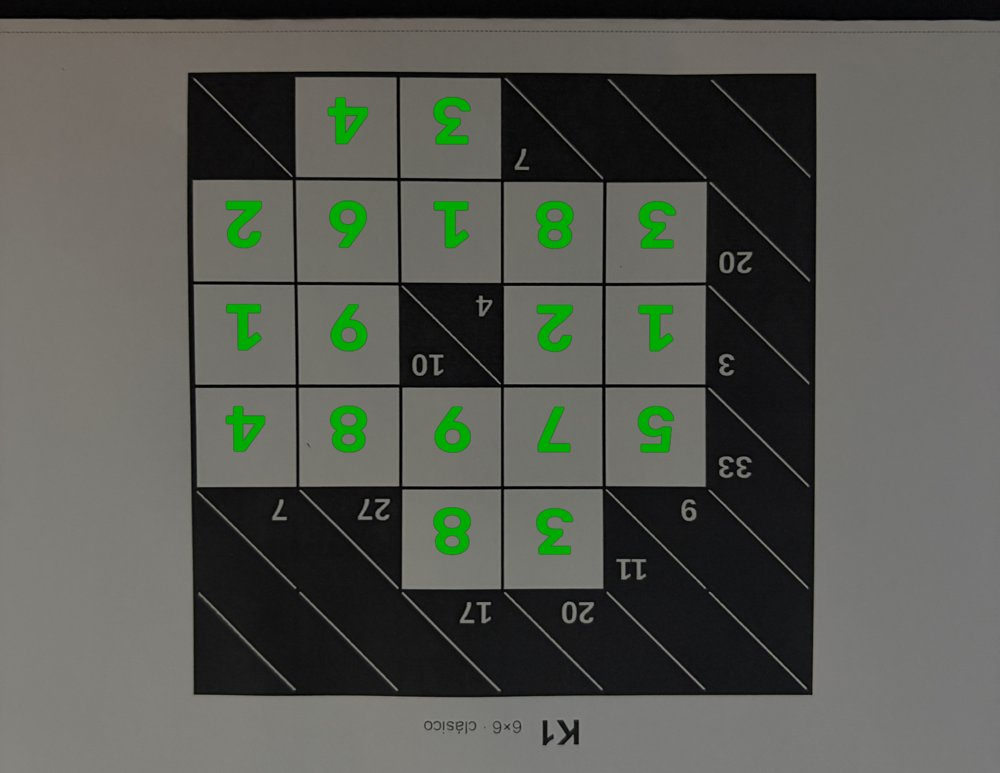
\includegraphics[width=0.48\columnwidth]{figs/sol_volteada.jpg}}\hfil
\subfloat[Ángulo fuerte (K4); el solver reparó una pista.]{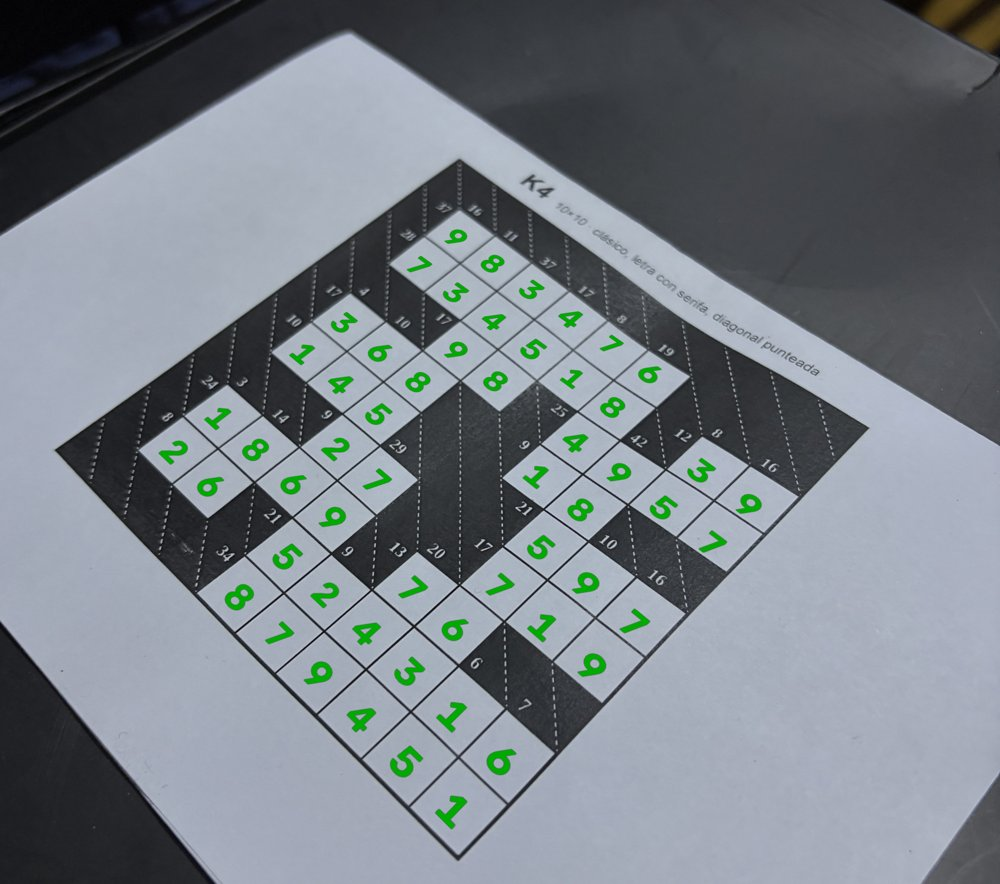
\includegraphics[width=0.48\columnwidth]{figs/sol_angulo.jpg}}
\caption{Solución dibujada por el sistema sobre fotos reales de tableros impresos.}
\label{fig:sol}
\end{figure}

\section{Datos}\label{sec:datos}
\subsection{Entrenamiento: datos sintéticos}
No existe un dataset público de imágenes de Kakuro etiquetadas, por lo que se aplica \emph{domain randomization}~\cite{tobin}:
\begin{enumerate}
  \item Se generan tableros aleatorios válidos (patrón aleatorio + relleno por backtracking sin repetir dígitos por corrida $\Rightarrow$ sumas).
  \item Se dibujan con 10 fuentes libres en \textbf{5 estilos visuales}: clásico (pistas negras, texto blanco), gris (pistas grises, texto negro),
        invertido de app (celdas a rellenar negras, pistas grises), triángulo blanco/negro y color. Se varían el tamaño de celda (36--90\,px),
        el grosor de línea, la diagonal (continua o punteada), la sombra y el margen.
  \item Se simula una foto: hoja sobre un fondo texturizado, perspectiva (hasta 8\% del lado por esquina), rotación ($\pm$12°), tinte de luz,
        gradiente de iluminación, desenfoque, ruido gaussiano, reescalado y compresión JPEG (calidad 35--95).
  \item Cada imagen pasa por \textbf{el mismo pipeline} de inferencia; como la suma real se conoce, cada recorte queda etiquetado automáticamente.
        Si el número de dígitos segmentados no coincide con la etiqueta, el recorte se descarta.
\end{enumerate}
Con 2500 tableros se obtuvieron 63\,078 dígitos (90\% entrenamiento / 10\% validación). Ninguna imagen de prueba se usa para entrenar.

\subsection{Dataset de prueba (\texttt{data/test\_set/})}
\begin{figure*}[!t]
\centering
\subfloat[Digitales, fotos simuladas, imprimibles y capturas de app (33 imágenes).]{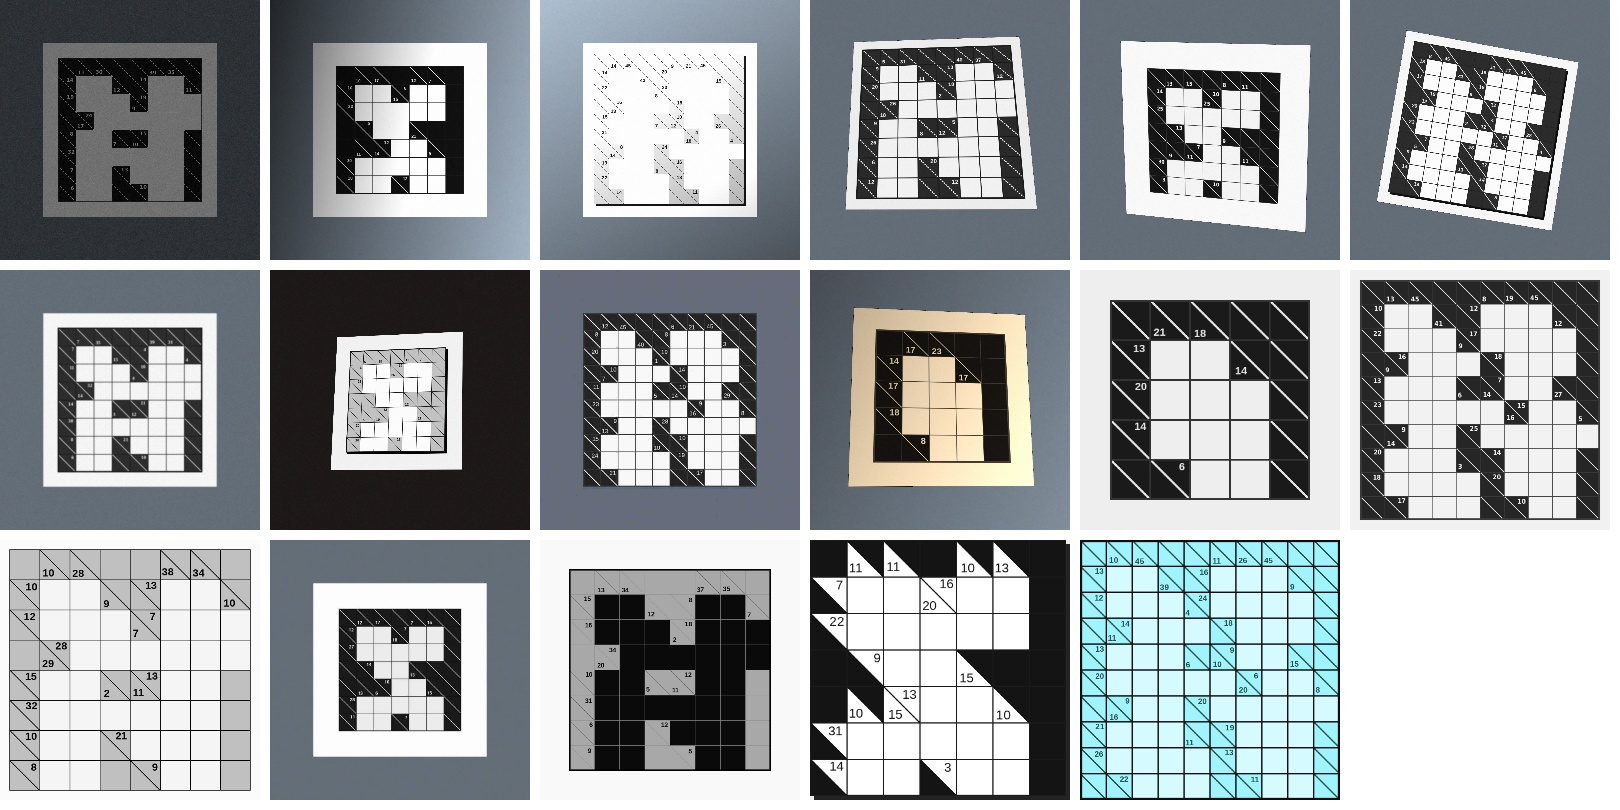
\includegraphics[width=\textwidth]{figs/test_set.jpg}}\\
\subfloat[Fotos de tableros impresos, una por condición (22 en total): frontal, ángulo, poca luz, sombra, volteada con sombra y flash.]{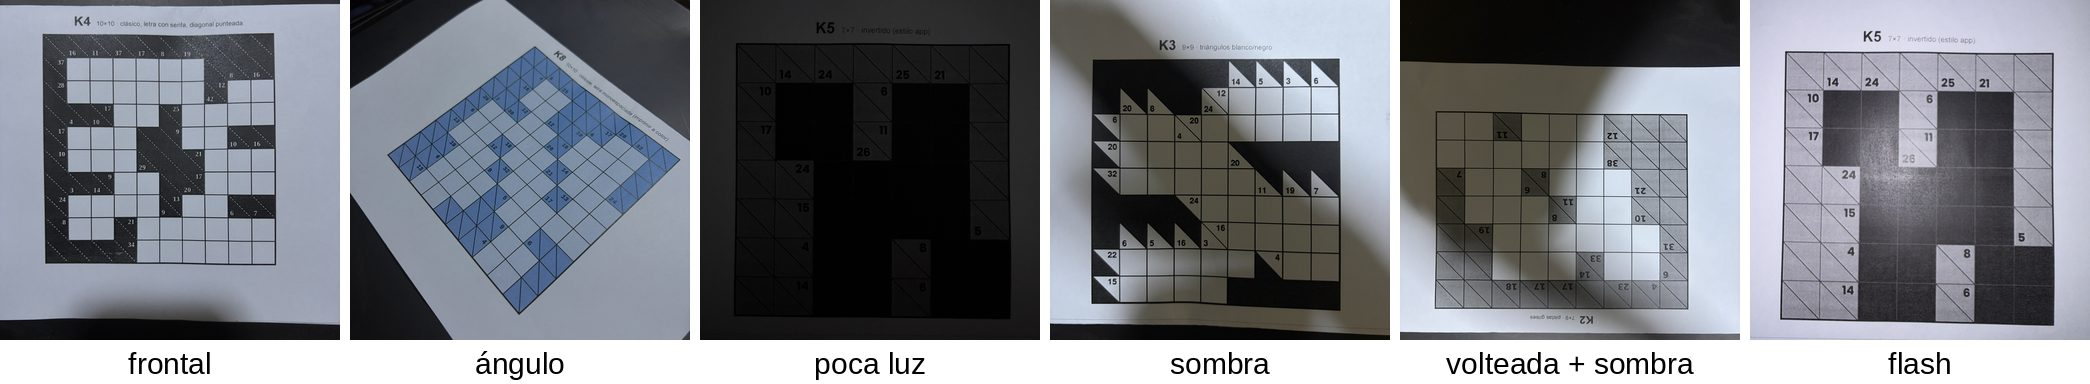
\includegraphics[width=\textwidth]{figs/fotos_condiciones.jpg}}
\caption{Dataset de prueba: 55 imágenes en cinco grupos.}
\label{fig:testset}
\end{figure*}
El enunciado exige al menos 10 imágenes en distintas condiciones, digitales e impresas. El dataset tiene 55, en cinco grupos
(Fig.~\ref{fig:testset}):
\begin{itemize}
  \item \textbf{Digitales (4)}: render limpio 5$\times$5 y 10$\times$10, estilo gris 8$\times$8 y una captura reducida al 55\% con compresión JPEG (7$\times$7).
  \item \textbf{Fotos simuladas (10)}: una condición controlada por imagen: luz baja, sombra lateral, reflejo brillante, ángulo leve,
        ángulo fuerte, rotación 10°, desenfoque, fondo oscuro, JPEG fuerte (calidad 25) y luz cálida.
  \item \textbf{Imprimibles (8)}: las páginas A4 de \texttt{printables/kakuro\_para\_imprimir.pdf} renderizadas a 300\,dpi
        (imágenes digitales, no fotografiadas), de 5$\times$5 a 10$\times$10, estilos clásico y gris.
  \item \textbf{Capturas de app (11)}: capturas de pantalla de una aplicación de Kakuro en el celular, de 7$\times$7 a 16$\times$14, que no fueron
        generadas por nosotros. Incluyen 6 estilos visuales: clásico, triángulo blanco/negro, amarillo, gris con diagonal punteada,
        gris claro con margen y el estilo \emph{invertido} (celdas a rellenar negras, pistas grises y un recuadro azul de selección).
        La aplicación no exporta la solución, así que la referencia se obtuvo con el pipeline y se verificó visualmente pista por pista
        (408 pistas).
  \item \textbf{Fotos de tableros impresos (22)}: siete tableros propios con solución única (K1--K6 y K8, de $6\times6$ a $12\times12$, en
        los estilos clásico, gris, triángulos, invertido y celeste, con letra con serifa o diagonal punteada en algunos) se imprimieron en
        A4 y se fotografiaron con un celular en seis condiciones: frontal (7), ángulo fuerte con la hoja girada (7), poca luz (2), sombra
        dura (3), hoja volteada 180° (2, una de ellas con sombra) y flash (1). Se publican sin metadatos de ubicación. La referencia de cada
        foto es la clave de respuesta del tablero impreso, así que es independiente del pipeline (\texttt{fotos\_impresas/}).
\end{itemize}
Los tres primeros grupos se generan con \texttt{python -m scripts.make\_test\_set}, con semillas distintas de las de entrenamiento;
sus tableros son válidos pero tienen más de una solución, lo que basta para evaluar la extracción.

\section{Resultados}\label{sec:res}
\subsection{Extracción (Fase 1)}
Métricas: \emph{grid} = filas$\times$columnas correctas; \emph{celdas} = blanca/no blanca correcta;
\emph{pistas} = valor exacto por (celda, dirección); \emph{exacto} = tablero sin ningún error;
\emph{resuelto} = el solver, con el JSON extraído, produce una solución válida del tablero real.
La Tabla~\ref{tab:vision} resume los resultados (\texttt{python -m scripts.benchmark vision -{}-dir data/test\_set/<grupo>}).

\begin{table*}[!t]
\centering
\caption{Resultados de extracción con la CNN (\%) y tiempo medio por imagen (CPU de 2 núcleos virtuales).}
\label{tab:vision}
\begin{tabular}{lccccccc}
\toprule
Conjunto & Imágenes & Grid & Celdas & Pistas & Exacto & Resuelto & Tiempo (s)\\
\midrule
Digitales & 4 & 100 & 100 & 100 & 100 & 100 & 2.2\\
Fotos simuladas & 10 & 100 & 100 & 100 & 100 & 100 & 1.5\\
Imprimibles (render digital) & 8 & 100 & 100 & 100 & 100 & 100 & 1.3\\
Capturas de app & 11 & 100 & 100 & 100 & 100 & 100 & 0.4\\
Fotos de tableros impresos & 22 & 100 & 98.7 & 95.6 & 81.8 & 81.8 & 1.2\\
\midrule
\textbf{Total dataset de prueba} & \textbf{55} & \textbf{100} & \textbf{99.5} & \textbf{98.3} & \textbf{92.7} & \textbf{92.7} & \\
\midrule
Sintético aleatorio (estrés) & 100 & 91.0 & 90.5 & 85.1 & 71.0 & 71.0 & 1.2\\
\bottomrule
\end{tabular}
\end{table*}

\noindent La precisión de la CNN en validación es \textbf{98.6\%}, medida sobre recortes sintéticos de dígitos, no sobre fotos. El conjunto
``sintético aleatorio'' usa la misma aumentación agresiva del entrenamiento (celdas pequeñas, contraste muy bajo, los 5 estilos) con
100 tableros nuevos, y sirve como prueba de estrés: la mayoría de sus errores son pistas casi ilegibles incluso para una persona.

La diferencia de tiempos se debe a la búsqueda de orientación. Si la primera lectura da un Kakuro con solución única y sin avisos,
se acepta sin probar las otras rotaciones; es lo que ocurre con las capturas de app. Los tableros generados por nuestro script tienen
más de una solución, así que no cumplen esa condición y se leen en las 4 orientaciones.

\subsection{Fotos reales por condición}
La Tabla~\ref{tab:fotos} compara las 22 fotos antes y después de los ajustes de robustez de la Fase~1: orden de esquinas por ángulo,
búsqueda de orientación, ajuste de la grilla por tramos, umbrales locales en escala logarítmica, suavizado del grano y reparación con
el solver. Antes, ninguna foto en ángulo se leía: con la hoja girada, ordenar las esquinas por $x+y$ y $y-x$ podía repetir un vértice
(la homografía degeneraba) y además el tablero quedaba rotado 90°; el orden por ángulo y la búsqueda de orientación resuelven ambos
casos. Las sombras pasan del 61.8\% al 90.9\% de pistas correctas. Siguen fallando 4 fotos: la volteada
con sombra (K2), las sombras más duras sobre K4 y K6, y el flash, cuyo reflejo altera el contraste de las celdas del estilo invertido;
es la única condición que empeora levemente (de 13 a 12 pistas).

\begin{table}[!t]\centering
\caption{Fotos de tableros impresos por condición, antes $\rightarrow$ después de los ajustes de robustez.}
\label{tab:fotos}
\begin{tabular}{lccc}
\toprule
Condición & Fotos & Exactos & Pistas (\%)\\
\midrule
Frontal & 7 & 5 $\rightarrow$ 7 & 97.9 $\rightarrow$ 100\\
Ángulo & 7 & 0 $\rightarrow$ 7 & 0 $\rightarrow$ 100\\
Poca luz & 2 & 2 $\rightarrow$ 2 & 100 $\rightarrow$ 100\\
Sombra & 3 & 1 $\rightarrow$ 1 & 61.8 $\rightarrow$ 90.9\\
Volteada & 2 & 0 $\rightarrow$ 1 & 0 $\rightarrow$ 65.6\\
Flash & 1 & 0 $\rightarrow$ 0 & 81.2 $\rightarrow$ 75.0\\
\midrule
Total & 22 & 8 $\rightarrow$ 18 & 52.1 $\rightarrow$ 95.6\\
\bottomrule
\end{tabular}
\end{table}

\subsection{OCR frente a correcciones del dominio}
Para separar lo que lee la CNN de lo que corrigen las reglas: en las 18 fotos exactas, la CNN leyó bien de forma directa 448 de sus
450 pistas. Las otras 2 las corrigió el solver: en K8 (frontal), un 16 leído en lugar de 6 dejaba el tablero sin solución; en K4 (ángulo),
un 73 imposible se reemplazó primero por la alternativa factible 23 y luego el solver lo llevó a 25, el valor correcto. En total, la
reparación con el solver cambió 2 pistas en 22 fotos y ambas quedaron bien. La regla de sumas factibles actuó 10 veces: una en K4, y
nueve en las fotos que fallan, donde una celda mal clasificada alteraba la longitud de la corrida; en 6 de esos 9 casos la CNN había
leído bien el número y la regla lo cambió. Es decir, en esas fotos la causa de fondo es la clasificación de celdas, no el OCR.

\subsection{Comparación con Tesseract}
Con una versión anterior del pipeline (sin búsqueda de orientación ni reparación con el solver), Tesseract leyó el 86.7\% de las
pistas de las fotos simuladas frente al 100\% de la CNN, y sólo 1 de las 11 capturas de app quedó sin errores frente a 11 de 11.
La mayor diferencia aparece con desenfoque, donde Tesseract leyó sólo 4 de 22 pistas. Además la CNN es unas 20 veces más rápida en el OCR.

\subsection{Robustez a estilos reales}
Las capturas de app y las fotos impresas difieren del generador en fuentes, colores, proporciones e iluminación. Las decisiones que
permiten leerlas son generales, no específicas de cada imagen: la búsqueda conjunta de (inicio, fin, $n$) de la grilla, la escala de
grises por PCA del color, el color a rellenar deducido por la regla de la primera fila y columna, la polaridad por triángulo con
eliminación de diagonales continuas o punteadas, los umbrales locales y el entrenamiento con los 5 estilos sintéticos.

\subsection{Comparación de modelos CP (Fase 2)}
La Tabla~\ref{tab:solver} compara las dos formulaciones (\texttt{python -m scripts.benchmark solver -{}-count 3}). Las \emph{ramas} cuentan las decisiones de búsqueda y los \emph{conflictos},
las ramas que terminaron en contradicción. El modelo global es más rápido en los cuatro patrones. La tabla propaga más dentro de cada
corrida (en el patrón de $7\times7$ resuelve sin ramificar), pero construir y propagar tablas grandes cuesta más: en $10\times10$ tarda
unas 7 veces más. Los tableros de este benchmark se generan rellenando el patrón al azar y tienen varias soluciones, por eso hay
búsqueda; en los 23 tableros con solución única ambos modelos resuelven con 0 ramas. CP-SAT usa 8 hilos en paralelo, así que las ramas
y los tiempos varían un poco entre corridas.

\begin{table}[!t]\centering
\caption{Modelo global frente al de tabla: promedio de 3 tableros aleatorios por patrón.}
\label{tab:solver}
\begin{tabular}{lcccccc}\toprule
 & \multicolumn{3}{c}{\texttt{AllDifferent} + suma} & \multicolumn{3}{c}{Tabla}\\
Patrón & s & ramas & confl. & s & ramas & confl.\\\midrule
5$\times$5 & 0.016 & 515 & 0.7 & 0.060 & 875 & 0.0\\
7$\times$7 & 0.010 & 186 & 0.0 & 0.011 & 0 & 0.0\\
8$\times$8 & 0.024 & 1347 & 5.3 & 0.067 & 3392 & 10.3\\
10$\times$10 & 0.052 & 2556 & 20.0 & 0.349 & 7687 & 4.7\\\bottomrule
\end{tabular}
\end{table}

\section{Limitaciones}
\begin{itemize}
  \item Se asume que el tablero es el objeto con más líneas de la imagen y que está completo dentro de la foto.
  \item Las sombras duras y el reflejo del flash todavía fallan (4 de 22 fotos): alteran la clasificación de celdas y, con ella, la
        longitud de las corridas, y entonces la regla de sumas factibles puede empeorar lecturas correctas.
  \item La reparación con el solver sólo detecta errores que dejan el tablero sin solución: una pista mal leída que siga siendo
        resoluble no se detecta.
  \item Fuentes muy decorativas o escritura a mano no están en el entrenamiento; se pueden incorporar con \texttt{-{}-real-dir}.
  \item Pliegues fuertes del papel (distorsión no proyectiva) sólo se corrigen parcialmente con el ajuste por tramos de la grilla.
  \item Las capturas de app no tienen una solución oficial: su referencia se obtuvo con el pipeline y se verificó visualmente. La
        evaluación independiente más exigente es la de las fotos impresas.
\end{itemize}

\section{Conclusiones}
El sistema cumple el flujo completo foto $\rightarrow$ JSON $\rightarrow$ CP $\rightarrow$ solución dibujada. La visión lee sin errores
las 33 imágenes digitales, simuladas y capturas de app, y el 95.6\% de las pistas de 22 fotos reales de tableros impresos (18 tableros
exactos); los ajustes de robustez subieron los tableros exactos de 8 a 18. El modelo CP es pequeño, con una variable por celda blanca y
dos restricciones globales por corrida, y gracias a la propagación resuelve y prueba la unicidad de los tableros con solución única sin
ramificar. No necesita restricciones reificadas porque todas las restricciones del Kakuro son incondicionales. Además, el modelo CP sirve
para validar la visión: orienta la hoja y repara lecturas sin solución. Como trabajo futuro proponemos entrenar con fotos reales con
sombras duras y flash, y modelar la incertidumbre del OCR dentro del solver con restricciones reificadas.

\begin{thebibliography}{9}
\bibitem{opencv} G.~Bradski, ``The OpenCV Library,'' \emph{Dr. Dobb's Journal of Software Tools}, 2000.
\bibitem{otsu} N.~Otsu, ``A threshold selection method from gray-level histograms,'' \emph{IEEE Trans. Syst., Man, Cybern.}, vol.~9, no.~1, pp.~62--66, 1979.
\bibitem{lecun} Y.~LeCun, L.~Bottou, Y.~Bengio, and P.~Haffner, ``Gradient-based learning applied to document recognition,'' \emph{Proc. IEEE}, vol.~86, no.~11, pp.~2278--2324, 1998.
\bibitem{tesseract} R.~Smith, ``An overview of the Tesseract OCR engine,'' in \emph{Proc. ICDAR}, 2007, pp.~629--633.
\bibitem{tobin} J.~Tobin \emph{et al.}, ``Domain randomization for transferring deep neural networks from simulation to the real world,'' in \emph{Proc. IROS}, 2017.
\bibitem{pytorch} A.~Paszke \emph{et al.}, ``PyTorch: An imperative style, high-performance deep learning library,'' in \emph{Proc. NeurIPS}, 2019.
\bibitem{ortools} L.~Perron and V.~Furnon, ``OR-Tools CP-SAT,'' Google. [Online]. Available: \url{https://developers.google.com/optimization}
\bibitem{regin} J.-C.~Régin, ``A filtering algorithm for constraints of difference in CSPs,'' in \emph{Proc. AAAI}, 1994, pp.~362--367.
\bibitem{rossi} F.~Rossi, P.~van~Beek, and T.~Walsh, Eds., \emph{Handbook of Constraint Programming}. Elsevier, 2006.
\end{thebibliography}
\end{document}
